%% LyX 2.1.3 created this file.  For more info, see http://www.lyx.org/.
%% Do not edit unless you really know what you are doing.
\documentclass[12pt,english]{article}
\usepackage[latin9]{inputenc}
\usepackage{color}
\usepackage{amsthm}
\usepackage{amsmath}
\usepackage{graphicx}

\makeatletter
%%%%%%%%%%%%%%%%%%%%%%%%%%%%%% Textclass specific LaTeX commands.
\numberwithin{equation}{section}
\numberwithin{figure}{section}

%%%%%%%%%%%%%%%%%%%%%%%%%%%%%% User specified LaTeX commands.
\usepackage[margin=0.75in]{geometry} % see geometry.pdf on how to lay out the page. There's lots.
\usepackage{graphicx}
\usepackage{cleveref}
\usepackage{amsmath}
\usepackage{multirow}
\usepackage{listings}
\usepackage{color}
\usepackage{CJK}
\definecolor{mygreen}{RGB}{28,172,0}
\definecolor{mylilas}{RGB}{170,55,241}

\usepackage[latin9]{inputenc}
\usepackage{geometry}
\geometry{verbose}


\makeatletter
\@ifundefined{date}{}{\date{}}
\makeatother

%Fancy-header package to modify header/page numbering 
\usepackage{fancyhdr}
\pagestyle{fancy}
\lhead{\textbf{Ge/ESE 118}} %name of the course
\chead{\textbf{}} %topic of the homework set
\rhead{\textbf{Solution 2}} %number of the homework set
\lfoot{}
\cfoot{}
\rfoot{\thepage}


% Matlab script
\lstset{language=Matlab,%
      %basicstyle=\color{red},
  breaklines=true,%
  morekeywords={matlab2tikz},
  keywordstyle=\color{blue},%
  morekeywords=[2]{1}, keywordstyle=[2]{\color{black}},
  identifierstyle=\color{black},%}
  stringstyle=\color{mylilas},
  commentstyle=\color{mygreen},%
  showstringspaces=false,%without this there will be a symbol in the places where there is a space
  numbers=left,%
  numberstyle={\tiny \color{black}},% size of the numbers
  numbersep=9pt, % this defines how far the numbers are from the text
  emph=[1]{for,end,break},emphstyle=[1]\color{red}, %some words to emphasise
                                                      %emph=[2]{word1,word2}, emphstyle=[2]{style},    
}

\makeatother

\usepackage{babel}
\begin{document}

\section*{Problem 1 (graded by Kangchen) - 50 points+10 bonus points}


\subsection*{(a)10 points}

The model parameter vector $\boldsymbol{m}=[x_{s},y_{s},z_{s},P]^{T}$.
The forward model is nonlinear, since the partial derivatives $\frac{\partial G}{\partial m_{i}}$
are not constant.


\subsection*{(b)10 points}

For least squares problem, we introduce the objective function:

\textcolor{blue}{\tiny{}
\[
F=\frac{1}{2}(\boldsymbol{d-g}(\boldsymbol{m}))^{T}(\boldsymbol{d-g}(\boldsymbol{m}))=\underset{}{\overset{n}{\frac{1}{2}\underset{i=1}{\sum}}(d_{i}-\frac{Pz_{s}}{[(x_{s}-x_{i})^{2}+(y_{s}-y_{i})^{2}+z_{s}^{2}]^{3/2}})^{2}}
\]
}{\tiny \par}

define : \textcolor{blue}{\tiny{}
\[
\eta_{i}=(x_{s}-x_{i})^{2}+(y_{s}-y_{i})^{2}+z_{s}^{2}
\]
 }{\tiny \par}

\textcolor{blue}{\tiny{}
\[
lx_{i}=x_{i}-x_{s}
\]
 }{\tiny \par}

\textcolor{blue}{\tiny{}
\[
ly_{i}=y_{i}-y_{s}
\]
}{\tiny \par}

\textcolor{blue}{\tiny{}
\[
A_{i}=d_{i}-\frac{Pz_{s}}{[(x_{s}-x_{i})^{2}+(y_{s}-y_{i})^{2}+z_{s}^{2}]^{3/2}}
\]
}{\tiny \par}

We write the $\hat{\boldsymbol{G}}$ matrix: \textcolor{blue}{\tiny{}
\[
\hat{\boldsymbol{G}}=\boldsymbol{\nabla}_{\boldsymbol{m}}G=\frac{\partial G_{i}}{\partial m_{j}}
\]
 
\[
\hat{\boldsymbol{G}}=\begin{bmatrix}\frac{3Pz_{x}lx_{1}}{2\eta_{1}^{5/2}} & \frac{3Pz_{x}ly_{1}}{2\eta_{1}^{5/2}} & \frac{PR_{1}-3Pz_{s}^{2}}{2\eta_{1}^{5/2}} & \frac{z_{s}}{2\eta_{1}^{3/2}}\\
\frac{3Pz_{x}lx_{2}}{2\eta_{2}^{5/2}} & \frac{3Pz_{x}ly_{2}}{2\eta_{2}^{5/2}} & \frac{PR_{2}-3Pz_{s}^{2}}{2\eta_{2}^{5/2}} & \frac{z_{s}}{2\eta_{2}^{3/2}}\\
... & ... & ... & ...\\
\frac{3Pz_{x}lx_{n}}{2\eta_{n}^{5/2}} & \frac{3Pz_{x}ly_{n}}{2\eta_{n}^{5/2}} & \frac{PR_{n}-3Pz_{s}^{2}}{2\eta_{n}^{5/2}} & \frac{z_{s}}{2\eta_{n}^{3/2}}
\end{bmatrix}
\]
}{\tiny \par}

\textcolor{blue}{\tiny{}
\[
\boldsymbol{\nabla_{m}}F=(\boldsymbol{d-g}(\boldsymbol{m}))^{T}\hat{\boldsymbol{G}}=[\underset{i=1}{\overset{n}{\sum}(}\frac{Pz_{s}}{\eta_{i}^{3/2}}-d_{i})(\frac{3Pz_{x}lx_{i}}{\eta_{i}^{5/2}}),\underset{i=1}{\overset{n}{\sum}(}\frac{Pz_{s}}{\eta_{i}^{3/2}}-d_{i})(\frac{3Pz_{x}ly_{i}}{\eta_{i}^{5/2}}),\underset{i=1}{\overset{n}{\sum}}(\frac{Pz_{s}}{\eta_{i}^{3/2}}-d_{i})(\frac{PR_{i}-3Pz_{s}^{2}}{\eta_{i}^{5/2}}),\underset{i=1}{\overset{n}{\sum}}(\frac{Pz_{s}}{\eta_{i}^{3/2}}-d_{i})(\frac{z_{s}}{\eta_{i}^{3/2}})]^{T}
\]
}{\tiny \par}

\textcolor{blue}{\tiny{}
\[
\boldsymbol{H}(F)=\boldsymbol{\nabla_{m}}(\boldsymbol{\nabla_{m}}F)=\nabla(\hat{\boldsymbol{G}}^{T}(\boldsymbol{d}-\boldsymbol{g}(\boldsymbol{m})))=\hat{\boldsymbol{G}}^{T}\hat{\boldsymbol{G}}-(\boldsymbol{d}-\boldsymbol{g}(\boldsymbol{m}))^{T}\boldsymbol{Q}
\]
}{\tiny \par}

\textcolor{blue}{\tiny{}
\[
\boldsymbol{H}_{approximate}=\hat{\boldsymbol{G}}^{T}\hat{\boldsymbol{G}}
\]
}{\tiny \par}

\textcolor{blue}{\tiny{}
\[
(\boldsymbol{d}-\boldsymbol{g}(\boldsymbol{m}))^{T}\boldsymbol{Q}=\underset{i=1}{\overset{n}{\sum}}\frac{A_{i}}{\eta_{i}7/2}\begin{bmatrix}15Pz_{s}lx_{i}^{2}-3Pz_{s}\eta_{i} & 15Pz_{s}lx_{i}ly_{i} & 3Plx_{i}\eta_{i}-15Pz_{s}^{2}lx_{i} & 3z_{s}lx_{i}\eta_{i}\\
 & 15Pz_{s}ly_{i}^{2}-3Pz_{s}\eta_{i} & 3Ply_{i}\eta_{i}-15Pz_{s}^{2}ly_{i} & 3z_{s}dy_{i}\eta_{i}\\
sym &  & 15Pz_{s}^{3}-9Pz_{s}\eta_{i} & R_{i}^{2}-9z_{s}^{2}\eta_{i}\\
 &  &  & 0
\end{bmatrix}
\]
}{\tiny \par}

\textcolor{blue}{\tiny{}
\[
\begin{array}{cc}
H_{xx}=\text{\ensuremath{\underset{i}{\sum}}}9P^{2}lx_{i}{}^{2}z{}_{s}^{2}\eta_{i}^{-5}-15lx_{i}^{2}z_{s}A_{i}\eta_{i}^{-7/2}+3Pz_{s}A_{i}\eta_{i}^{-5/2} & H_{yy}=\text{\ensuremath{\underset{i}{\sum}}}9Ply_{i}{}^{2}z{}_{s}^{2}\eta_{i}^{-5}-15ly_{i}^{2}z_{s}A_{i}\eta_{i}^{-7/2}+3Pz_{s}A_{i}\eta_{i}^{-5/2}\\
H_{zz}=\text{\ensuremath{\underset{i}{\sum}}}(-6Pz_{s}^{2}\eta_{i}^{-5/2}+P\eta_{i}^{-3/2})^{2}-15A_{i}Pz_{s}^{3}\eta_{i}^{-7/2}+9A_{i}Pz_{s}\eta_{i}^{-5/2} & H_{pp}=\text{\ensuremath{\underset{i}{\sum}}}z_{s}^{2}\eta_{i}^{-3}\\
H_{xy}=\text{\ensuremath{\underset{i}{\sum}}}9P^{2}lx_{i}lyz_{i}{}_{s}^{2}\eta_{i}^{-5}-15lx_{i}ly_{i}z_{s}A_{i}\eta_{i}^{-7/2} & H_{xz}=\text{\ensuremath{\underset{i}{\sum}}}-3Plx_{i}A_{i}\eta_{i}^{-5/2}-15Plx_{i}z_{s}^{2}\eta_{i}^{-7/2}+3Plx_{i}z_{s}\eta_{i}^{-4}-9P^{2}lx_{i}z_{s}^{3}\eta_{i}^{-5}\\
H_{xp}=\text{\ensuremath{\underset{i}{\sum}}}3Plx_{i}z_{s}^{2}\eta_{i}^{-4}-3lx_{i}z_{s}A_{i}\eta_{i}^{-5/2} & H_{yz}=\text{\ensuremath{\underset{i}{\sum-}}}3Ply_{i}A_{i}\eta_{i}^{-5/2}-15Ply_{i}z_{s}^{2}\eta_{i}^{-7/2}+3P^{2}ly_{i}z_{s}\eta_{i}^{-4}-9Plx_{i}ly_{i}z_{s}\eta_{i}^{-5}\\
H_{yp}=\text{\ensuremath{\underset{i}{\sum}}}3Ply_{i}z_{s}^{2}\eta_{i}^{-4}-3ly_{i}z_{s}A_{i}\eta_{i}^{-5/2} & H_{zp}=\text{\ensuremath{\underset{i}{\sum}}}-3Pz_{s}^{3}\eta_{i}^{-4}+P_{i}z_{s}\eta_{i}^{-3}+3A_{i}z_{s}^{2}\eta_{i}^{-5/2}-A\eta_{i}^{-3/2}
\end{array}
\]
}{\tiny \par}

Note: this is the exact hessian, set $A_{i}=0$ will make the approximated
Hessian.

The algorithm for finding solution is :

$\boldsymbol{m}=\boldsymbol{m}_{0}$ (set initial guess)

$\boldsymbol{r}=(\boldsymbol{d}-\boldsymbol{g}(\boldsymbol{m}))$

while $\boldsymbol{r^{T}r}$\textgreater{}errorbound

......compute Hessian $\boldsymbol{H}(\boldsymbol{m})$ and $\hat{\boldsymbol{G}}^{T}\boldsymbol{r}$

......$\Delta\boldsymbol{m}=\boldsymbol{H}^{-1}\hat{\boldsymbol{G}}^{T}\boldsymbol{r}$

......$\boldsymbol{m}=\boldsymbol{m}+\Delta\boldsymbol{m}$

......$\boldsymbol{r}=(\boldsymbol{d}-\boldsymbol{g}(\boldsymbol{m}))$

end


\subsection*{(c)10 points}

\tiny
\lstinputlisting{compute_gradient_approx_hess.m}
\normalsize\tiny
\lstinputlisting{nonlinear_solver.m}
\normalsize\tiny
\lstinputlisting{compute_residue.m}
\normalsize\tiny
\lstinputlisting{HW2.m}
\normalsize


\subsection*{(d)10 points}

$[x_{s},y_{s},z_{s},P]^{T}=[8.137,-5.142,11.507,30.346]^{T}$


\subsection*{(e)10 points}

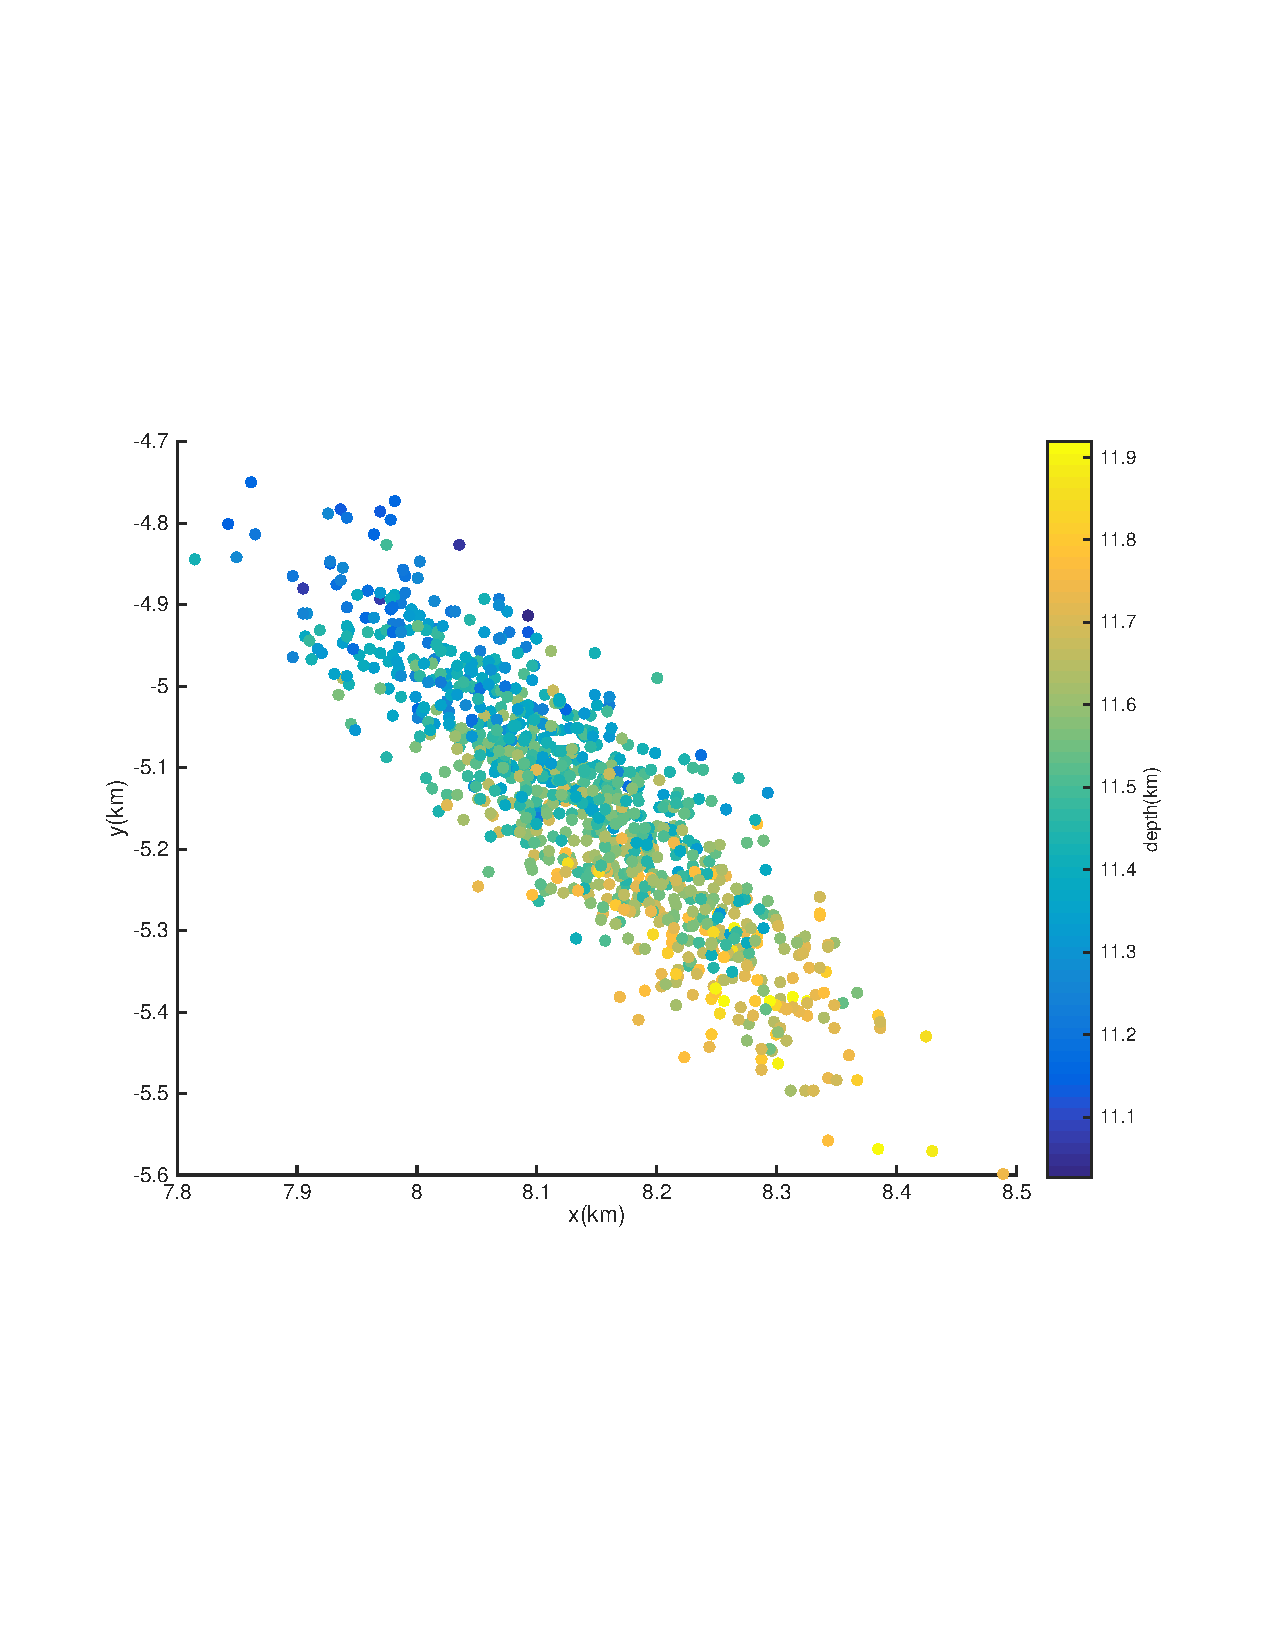
\includegraphics[scale=0.8]{measurements_error}

The standard deviations are $\sigma_{x_{s}}=0.099670,\sigma_{y_{s}}=0.137469,\sigma_{z_{s}}=0.149719,\sigma_{p}=0.691071$

There is a strong tradeoff relation between $x_{s},y_{s},z_{s}$.
$x_{s},y_{s}$ are negatively related. $x_{s},z_{s}$ are positively
related. $z_{s},y_{s}$ are negatively related. Note that we use $z_{s}$
as depth value. It is always non-negative.


\section*{Problem 2 (graded by Yiran) - 50 points}


\subsection*{(a) 4 points}

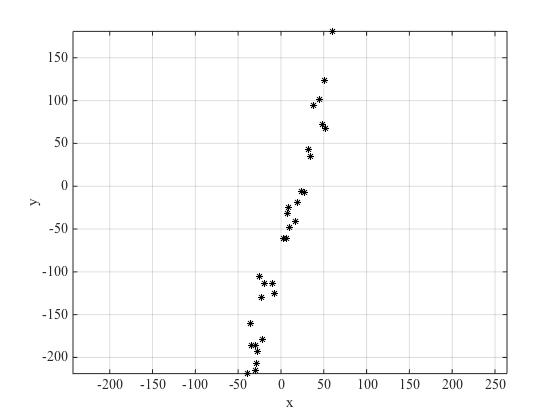
\includegraphics[scale=0.5]{p2_figures/p2a_data}


\subsection*{(b) 6 points}

$m_{1}$ is the intercept with the $y$ axis. From the plot, we estimate
that it should be bounded by $[-150,0]$. \\
$m_{2}$ is the slope of the line, we also estimate from the plot
that it should be bounded by $[1,10]$. \\
As suggested in the problem, the arrays are better no larger than
a few megabytes (1 double = 8 bytes) to avoid ``out of memory''
error. A 1000 by 1000 double-type matrix is 8 megabytes. Therefore,
we can choose the discretization as $m1=[-150:0.1:0]$, and $m2=[1:0.01:10]$,
so that the matrices of size length(m1) by length(m2) (e.g. the error
matrix plotted in (d)), will be in appropriate size.\\
We can always shrink our model space and do a finer search as following
steps.


\subsection*{(c) 6 points }

(See attached MATLAB code.)


\subsection*{(d) 10 points}

(See attached MATLAB code.)\\
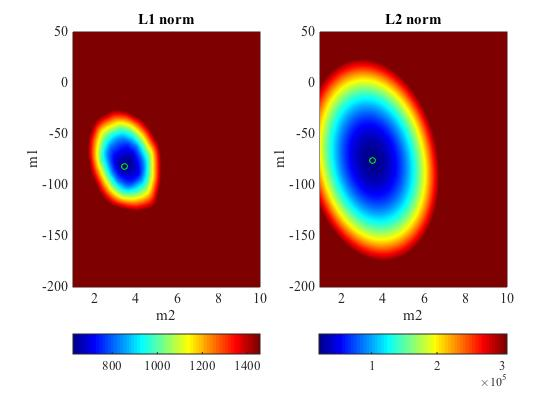
\includegraphics{p2_figures/p2d_misift}


\subsection*{(e) 4 points}

The solutions with lowest misifit are

L2 norm: (-75.5, 3.53)

L1 norm: (-81.9, 3.48)


\subsection*{(f) 10 points}

(See attached MATLAB code.)\\
The least square solution is: (-75.4631, 3.5301)


\subsection*{(g) 4 points}

From (d), we infer that the model parameters are negatively correlated,
and also the error is underestimated (much larger than 0.1). It is
not given in the standard result. The standard result gives the standard
deviations of each parameter, which are the diagonal terms of the
model convariance matrix. It will underestimate the range of possible
model parameters, if the model parameters are not independent, or
the data error is underestimated. Therefore, the extra information
given in (d) is also very important.


\subsection*{(h) 6 points}

(This is an open question.) \\
The L1 and L2 methods (``grid search'') are more straighforward
in showing the error distribution, thus the probability of the model
parameters over the ``full'' model space. \\
The least-square solution (``direct inversion'') is fast, and gives
the exact solution that minimizes L2 norm error. We can also infer
the covariances of the model parameters from the model covariance
matrix. However, it is not as straightforward, and sometimes gives
an illusion that the results have small errors/standard deviations.
In this small size problem, I would prefer the ``grid search'' method.\\
As the errors get bigger, the L1 norm method can be better, because
it would be less likely to be affected by the outliers. Moreover,
if there are several solutions that can minimize the error equally
well, we can see it in the error map produced by the direct search
method, and can choose one solution based on some priori information.
Therefore, I will prefer L1 norm.\\
\tiny
\lstinputlisting{hw2_2.m}
\normalsize
\end{document}
